%==============================================================================
% locality-performance.tex
%==============================================================================

\chapter{Performance}
\label{chap:locality-performance}

The performance results in this chapter are obtained on an Intel
Nehalem system with two processors and eight cores, running Ubuntu
9.04 64-bit with kernel 2.6.29 and Sun Hotspot JDK 1.6.0\_20 (Appendix
\ref{sec:experimental-setup-mafushi}). The JVM is invoked with the
following parameters:

\begin{lstlisting}[style=Listing]
  -server -Xmx4096M -Xms4096M -Xss8M -XX:+UseNUMA
\end{lstlisting}

It is important that our new scheduler implementation does not affect
the performance of existing locality-ignorant intervals
programs. Thus, we run the locality-ignorant JGF benchmarks (Appendix
\ref{chap:appendix-benchmarks}) with our new scheduler
implementation. As Figure \ref{fig:locality-evaluation-jgf} shows, the
performance of locality-ignorant JGF benchmarks on the locality-aware
intervals scheduler is comparable to the original implementation.

\begin{figure}[!ht]
  \centering
  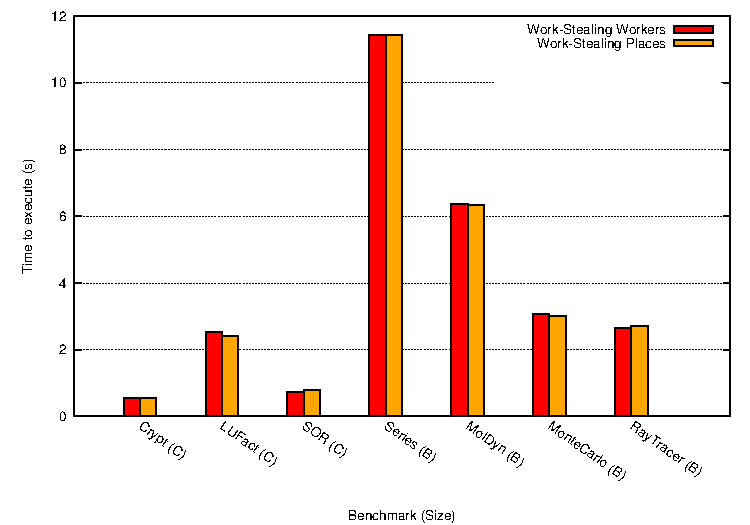
\includegraphics[width=0.6\linewidth]{locality-evaluation/mafushi-jgf}
  \caption[Locality-ignorant JGF benchmarks running on locality-aware
  scheduler]{Locality-ignorant JGF benchmarks using the locality-aware
    scheduler on our Intel Nehalem (Appendix
    \ref{sec:experimental-setup-mafushi}) test machine}
  \label{fig:locality-evaluation-jgf}
\end{figure}

The rest of this chapter evaluates the performance of the new
intervals scheduler on three different locality-aware benchmarks. To
reduce the impact of JVM overheads in the evaluation, the execution
time reported is the average of the three best from 10 benchmark
iterations.

\section{Cache-Stress Test}
\label{sec:locality-performance-cache-stress-test}

\todo{Describe benchmark ``Cache-Stress Test''}

\section{Merge Sort}
\label{sec:locality-performance-merge-sort}

\todo{Describe benchmark ``Merge Sort''}

\section{Block Matrix Multiplication}
\label{sec:locality-performance-block-matrix-multiplication}

\todo{Describe benchmark ``Block Matrix Multiplication''}

\todo{Finish chapter ``Performance''}


%%% Local Variables: 
%%% mode: latex
%%% TeX-master: "thesis"
%%% End: 
